\section{Evaluation}

When operating a service, the overall performance objective is to provide acceptable service latency at minimal cost. The cost can be lowered by running fewer servers - but this increases the latency because requests spend more time waiting for contended resources (such as network, storage, CPU, threads, locks, and so on). This tradeoff is an essential challenge for developers writing an elastic service application. 

To clarify the value that our mechanism provides to service architects, we now quantify both (a) its latency overhead and (b) its resource consumption, by comparing them to alternative solutions, including periodic polling (\S\ref{sec:polling}) and application-level change propagation (\S\ref{sec:observers}). To this end, we designed two series of experiments that measure low-load latency (\S\ref{sec:latency}), and variable-load throughput (\S\ref{sec:throughput}).

\paragraph{Application Model.}  
We model the application using  \emph{item} grains that are observed by \emph{view} grains. Each view's computation calls a configurable number of items, selected at random at the beginning of the test, either sequentially or in parallel. Varying the number of items and views can emphasize different aspects of an implementation. For example, a high \emph{fan-out} (= average number of views that depend on an item) means that whenever an item is mutated, many change propagation messages are sent to its views. We use the parameter combinations shown in Table~\ref{tab:param}.

\begin{table}
\begin{tabularx}{.99\columnwidth}{@{}Xrrr@{}} \toprule
Name		& \#items 	& \#views & \#dependencies \\ \midrule
low-load	&  600        	& 20       & 4  \\
fanout-1	& 20,000	& 20,000 & 1 \\
fanout-20	& 10,000	& 20,000 & 10 \\
fanout-200 & 1,000	& 20,000 & 10 \\  
\end{tabularx}
\caption{Named parameter combinations.}\label{tab:param}
\end{table}

\paragraph{Experimental Setup.} The grains are distributed over a Orleans cluster of five servers (silos) deployed as a Windows Azure cloud service. The load for the throughput experiments is generated by 10 servers. All processors have 8 cores, 14GB of RAM, and run at 1.6 GHz. To account for unexpected variations, we made sure to run each experiment series on at least 2 different datacenters, on at least 3 different days, and running the experiments in different order. Absolute numbers vary up to 10\%, but the relative performance of the various solutions, and thus the qualitative conclusions drawn, were stable. Note that we achieved this only after substantial work on our experiment framework. In particular for the thoughput experiments, a careful implementation of initialization and cleanup phases was important.

\subsection{Latency}\label{sec:latency}

Our latency experiments use the low-load parameters (Table~\ref{tab:param}) which avoids delays caused by queueing and contention. We measure two types, called \emph{query latency} and \emph{propagation latency}. Latencies are measured 4000 times each (200 times per view, separated by 500ms). We describe the results using the median and lower and upper quartiles.\footnote{Average and standard deviation are unsuitable statistics because of the long tail of the distribution.}

\subsubsection{Query Latency}


\begin{figure}
\begin{lstlisting}
grain View
{
	state Deps: Item[4]; 
	op Query(sequential: bool) : int[]
	{	
		var result = new int[4];
		if (sequential) {
			for (0 <= i < 4)
				result[i] = Deps[i].GetValue();
		} else {
			parallel for (0 <= i < 4)
				result[i] = Deps[i].GetValue();
		}
		return result;
	}
	op OneTimeReactiveQuery(sequential: bool) : int[]
	{
	 	var rc = CreateReactiveComputation(
	 										() => Query(sequential));
		var result = await rc.GetResultTracker.NextResult();
		rc.Dispose();
		return result;
	}
}
\end{lstlisting}
\caption{Pseudocode for the views in the latency experiments.}\label{fig:queries}
\end{figure}

\begin{figure}
\begin{tabular}{c}
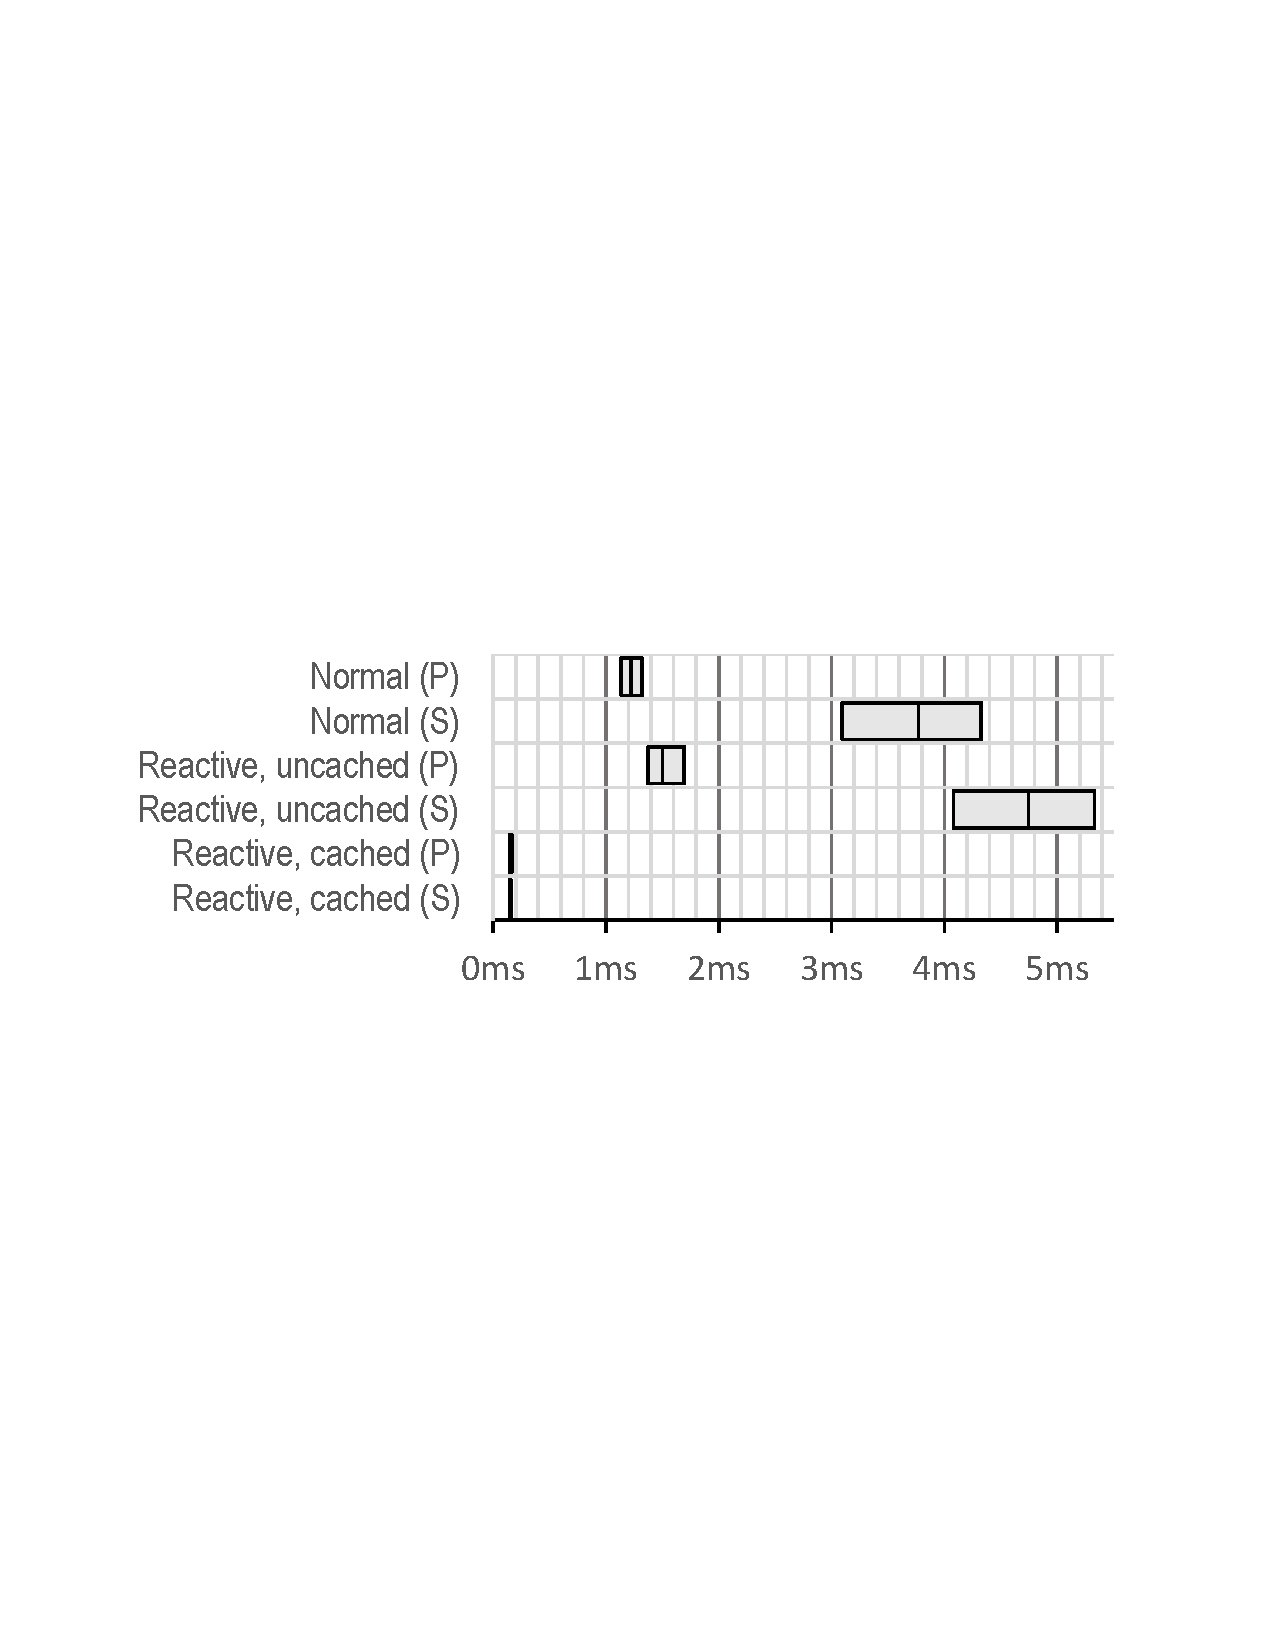
\includegraphics[width=\columnwidth, viewport=67 322 534 477]{figs/query-latencies}\\[.2in]
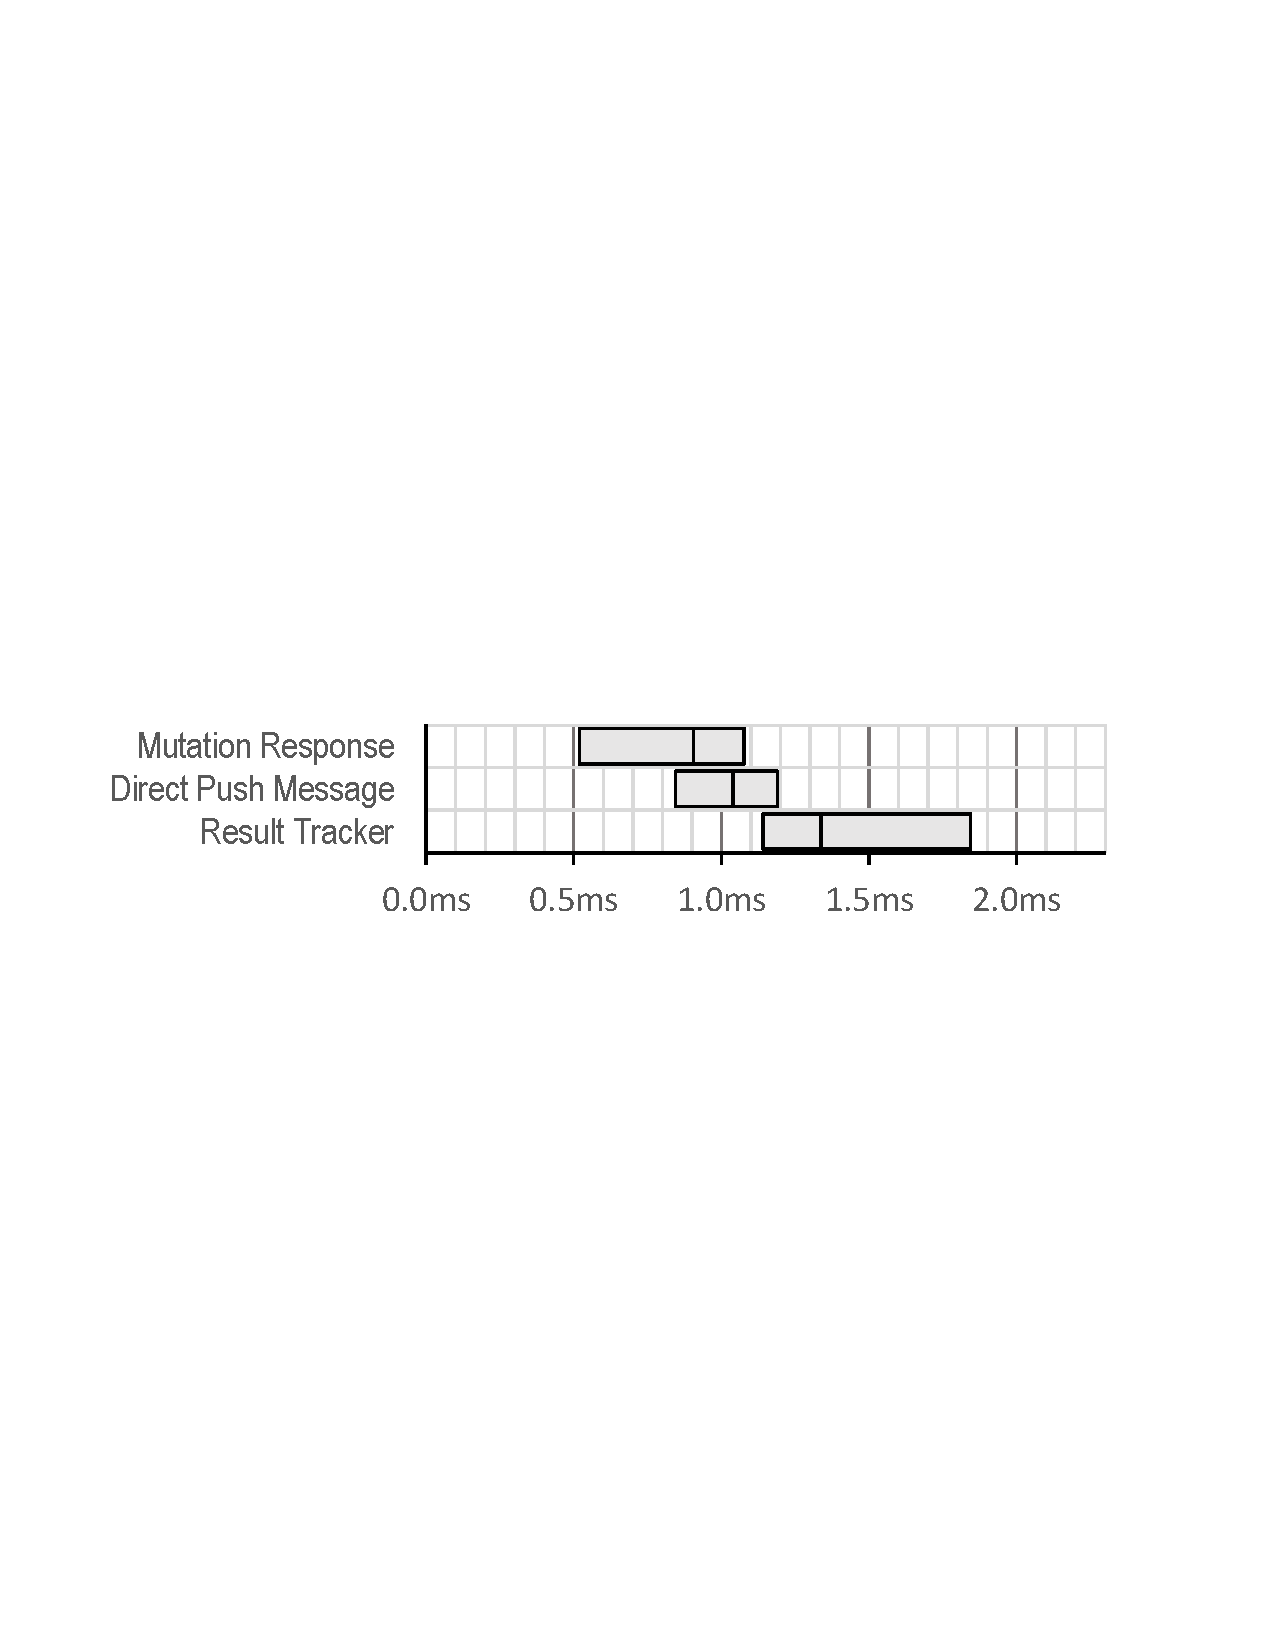
\includegraphics[width=\columnwidth, viewport=54 354 530 444]{figs/push-latencies}\\[.2in]
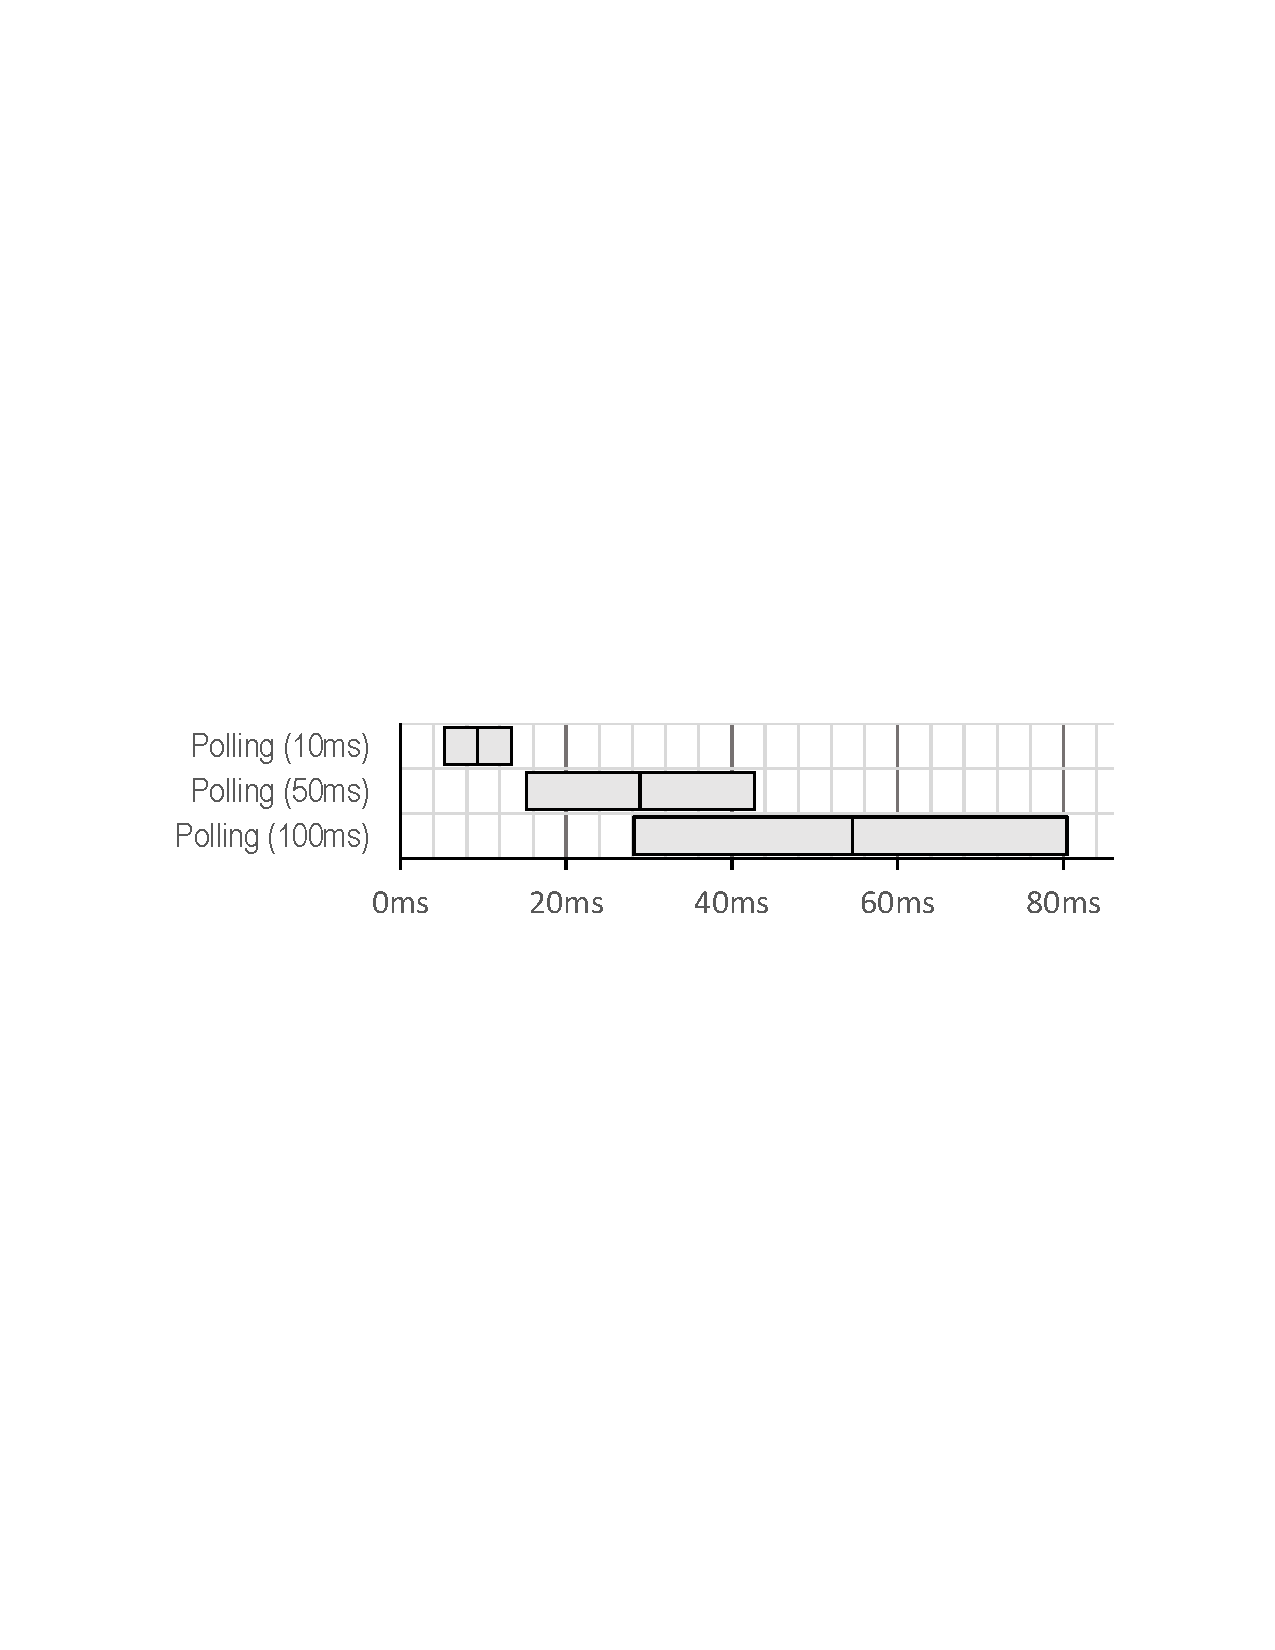
\includegraphics[width=\columnwidth, viewport=85 354 534 444]{figs/polling-latencies}\\
\end{tabular}
\caption{Measured latencies under low load, in milliseconds. The line in the middle of each box is the median, and the left and right edge are the first and third quartile. \textbf{(top)} Latencies for parallel and sequential queries; \textbf{(middle)} latencies for mutation response, application-level propagation using direct messages, and automatic propagation using result trackers; \textbf{(bottom)} propagation latencies for the polling solution at various frequencies}\label{fig:querylatencies}
\end{figure}

Consider a query executed on a view that calls each of four items (either sequentially or in parallel) to collect some value and returns the values in an array (Fig.~\ref{fig:queries}). We now compare the latency when executed normally (\lstinline|Query|) to the latency when executed as a reactive computation (\lstinline|OneTimeReactiveQuery|). The normal latency for the sequential and parallel versions are shown in the first two rows of Fig.~\ref{fig:querylatencies} (top). The median latency is about 1.2ms for the parallel query and 3.8ms for the sequential query. This is consistent with the round-trip time of a typical grain call taking a bit less than 1ms. For the reactive queries, we distinguish two cases. If  the relevant summaries are not already cached on the silo, the query takes about 25\% longer than normal (rows 2,3). This overhead is caused by the installation and removal of the summary caches, and by scheduling overhead of our reactive caching implementation. However, if summaries for the items are already cached on the silo (for example, if another view is tracking the same items), the latency of \lstinline|OneTimeReactiveQuery| is less than 200$\mu$s (rows 4,5) because remote calls can be completely avoided. 

These results demonstrate that (1) the latency overhead of constructing the dependency graph is modest, and (2) even if reactive tracking is not desired (here, the computation is executed once and then disposed), the caching effect alone can improve the service latency.


\subsubsection{Propagation Latency}

To provide reactive behavior, views should be updated whenever the items they depend on are mutated. We now measure the latency of this propagation for various solutions.

First, we measured the propagation speed of an application-level implementation where each item directly sends a notification message to all dependent views when mutated. This establishes a lower bound on how fast propagation can take in this environment, but can be quite challenging for developers to implement (as discussed in \S\ref{sec:observers}). The results show that the propagation message arrives right after the mutation completes: both take close to 1ms (rows 2,3 of Fig.~\ref{fig:querylatencies} (middle)). This is consistent with the underlying system sending the mutation response message and the propagation message at about the same time. 

For our proposed solution (using a reactive computation and a result tracker), the propagation takes about 300$\mu$s longer (row 3), reflecting the scheduling overhead of our change propagation implementation.

Finally, we looked at the propagation speed of a polling-based solution is much slower. Fig.~\ref{fig:querylatencies} (bottom) shows the measured latencies, using a sequential query and various polling intervals. As expected, we see a median propagation time in the neighborhood of half of the polling interval plus the query latency, and a wide inter-quartile distance. Note that polling as frequently as every 100ms is not advisable in practice (we show this in the throughput section). Reasonable polling intervals are more typically between 3 and 30 seconds, meaning that the median propagation speed is 1.5--15 seconds which is three orders of magnitude slower than for a reactive solution. 

The propagation latency results show that our proposed solution performs much better than a polling solution (while having the same simple programming model) and is largely competitive with a manual change propagation implementation (which is much harder to implement in general). 


\subsection{Throughput}\label{sec:throughput}